
\documentclass[11pt, aspectratio=43]{beamer}
\usepackage{templates/beamerthemeICube}
\usepackage{tikz}
\usetikzlibrary{matrix}

% Remove navigation bar
\setbeamertemplate{navigation symbols}{}
% Tikz package
\usepackage{tikz}
\usetikzlibrary{positioning}
\usepackage[export]{adjustbox}
\usepackage{booktabs}
\usepackage{siunitx}
\usepackage{amssymb}
\usepackage{xmpmulti}

\usepackage{graphicx}
\graphicspath{{figures/},{logos/}}


% Make links show up as coloured
\hypersetup{
  colorlinks = true,
  allcolors = black,
  urlcolor = blue,
}

\newcommand{\fullframeimage}[1]{
	\begin{center}%
		\includegraphics[max width = \textwidth, max height=0.8\textheight]{#1}%
	\end{center}
}

\newcommand{\ing}[1]{\includegraphics[width=2cm]{#1}}
\tikzset{
  % style for inserting images as nodes
  img/.style={
    text width=2cm,
    %text height=2cm,                 %% don't use this
    inner sep=0pt,     %% use this
    outer sep=0pt,     %% and this
    rectangle,
    align=center,
    draw,thick} % only for debugging..
}

%\let\emph\relax % there's no \RedeclareTextFontCommand
\DeclareTextFontCommand{\emph}{\color{slide-color}}

\colorlet{slide-color}{unistra}


\title{Laboratoire des sciences de l'ingénieur, de l'informatique et de l'imagerie}
\subtitle{ICube, UMR 7357}
\author{L. Barbé}
\institute{Plateforme Imagerie, Robotique et Innovation en Santé}
\date{\today}


% You can add any logos you like by uploading them into the logos folder and replacing the blank image here
\titleimage{image_fond.png}
\titlelogoa{unistra/signature-universite-minimale-couleur_03.png}
\titlelogob{cnrs/LOGO_CNRS_BLEU.png}
\titlelogoc{insa_strasbourg/Logo_INSAvilleStrasbourgCourt-pantone_marge.jpg}
\titlelogod{inria/inr_logo_rouge.png}
\titlelogoe{engees/ENGEES_CMJN_png.png}
%\titlelogoa{belle2-logo}
%\titlelogob{bmbf}
%\titlelogoc{blank}


% Bibliography
% Uncomment and upload your own references if you so please.
% \usepackage[citestyle=authoryear,bibstyle=numeric,hyperref,backend=biber]{biblatex}
% \addbibresource{references.bib}
% \bibhang1em

\begin{document}

\selectlanguage{french}

%\frame{\titlepage}
\begin{frame}[plain]
    \begin{tikzpicture}[remember picture,overlay]
    % Background image
    \node[above right, align=center,inner sep=0pt] at (current page.south west)
    {
        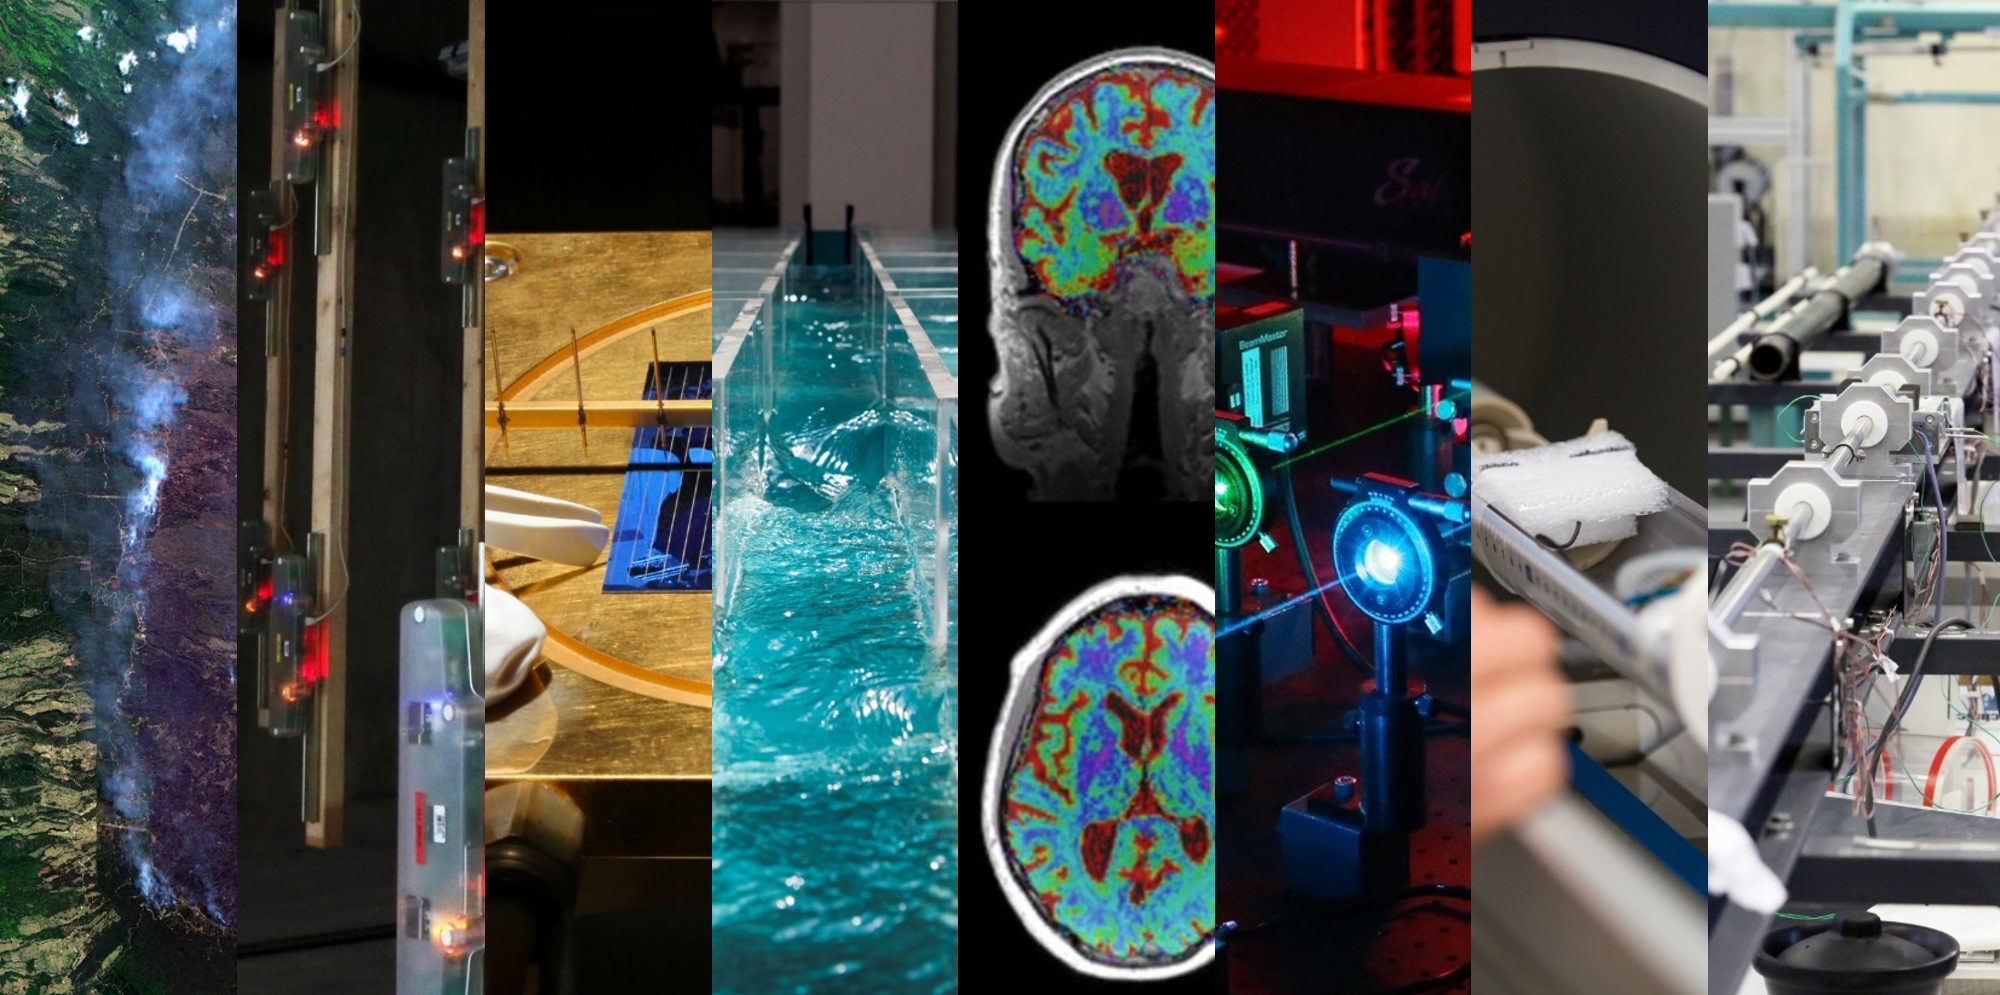
\includegraphics[width=0.95\paperwidth]{image_fond.png}
    };
        
    % Title & Subtitle
    \node
    [
        above=0.5cm,
        align=left,
        fill=unistra,
        rounded corners,
        inner xsep=15pt,
        inner ysep=10pt,
        minimum width=0.85\textwidth,
        text width=0.8\textwidth,
        fill opacity=0.7,
        text opacity=1,
        text=white
    ] (title) at (current page.center)
    {
        \Large \textbf{\inserttitle }  \\[5pt]
        \small \insertsubtitle
    };
    \node
    [
        below=0.5cm,
        align=left,
        fill=unistra,
        rounded corners,
        inner xsep=15pt,
        inner ysep=10pt,
        minimum width=0.7\textwidth,
        text width=0.6\textwidth,
        fill opacity=0.7,
        text opacity=1,
        text=white
    ] (subtitle) at (title.south)
    {
        \large \insertinstitute  \\[5pt]
    };
    % Author 
    \node[  below=0.5cm,        
            align=left,
            fill=unistra,
            rounded corners,
            inner xsep=15pt,
            inner ysep=10pt,
            minimum width=0.7\textwidth,
            text width=0.6\textwidth,
            fill opacity=0.7,
            text opacity=1,
            text=white
    ] (author) at (subtitle.south){\insertauthor};
    % Date
    \node[below=0.5cm,             
    align=left,
    fill=unistra,
    rounded corners,
    inner xsep=15pt,
    inner ysep=10pt,
    minimum width=0.7\textwidth,
    text width=0.6\textwidth,
    fill opacity=0.7,
    text opacity=1,
    text=white] (date) at (author.south){\large \today};
    % Logo

     \node
    [
        below right =0.25cm and 0.5cm
    ] at (current page.north west)
    {
         \includegraphics[height=1.5cm]{icube/icube-png.png}
    };
    \node
    [
        below left =0.25cm and 0.25cm
    ] at (current page.north east)
    {
        \includegraphics[height=0.6cm]{inria/inr_logo_rouge.png}
    };
    \node
    [
        below left =0.25cm and 2.2cm
    ] at (current page.north east)
    {
        \includegraphics[height=0.6cm]{engees/ENGEES_CMJN_png.png}
    };
    \node
    [
        below left =0.25cm and 3.5cm
    ] at (current page.north east)
    {
        \includegraphics[height=0.6cm]{insa_strasbourg/Logo_INSAvilleStrasbourgCourt-pantone_marge.jpg}
    };
    \node
    [
        below left =0.25cm and 5.0cm
    ] at (current page.north east)
    {
        \includegraphics[height=0.6cm]{cnrs/LOGO_CNRS_BLEU.png}
    };
    \node
    [
        below left =0.25cm and 6cm
    ] at (current page.north east)
     {
         \includegraphics[height=0.6cm]{unistra/signature-universite-minimale-couleur_03.png}
    };
    \end{tikzpicture}
    %\titlelogoe{}
\end{frame}

% One way to make a slide


\end{document}
